%   % !TEX root = ../../VIII,3_Rahmen-TeX_8-1.tex
%
%
%   Band VIII, 3 N.~??A45
%   Signatur/Tex-Datei: LH_37_05_045-046
%   RK-Nr. 60301
%   \ref{RK60301}
%   Überschrift: [Demonstratio de restitutionis elasticae isochronismo]
%   Modul: AEF / Elastizität
%   Datierung: ??? 1690 bis 1695 ???
%   WZ:
%.      (Bl. 45) LEd-WZ 803042 = RK-WZ 455, 514, 7e
%       (Bl. 46) LEd-WZ 803042, Gegenmarke = RK-WZ 560
%       (insgesamt: eins)
%   SZ:   (?????)
%   Bilddateien (PDF):
%      LH_37_05_045-046_d1 ((ex: lh037_05_045r-d1))
%      LH_37_05_045-046_d2 ((ex: lh037_05_045v-d1))
%      LH_37_05_045-046_d3 ((ex: lh037_05_046r-d1))
%      LH_37_05_045-046_d4 ((ex: lh037_05_046r-d2))
%      (insgesamt: vier)
%   Verzeichniseinträge: ????
%   \textls{} statt \textso{} (Ausnahme: Personenverzeichnis)
%
%
\selectlanguage{ngerman}%
\frenchspacing%
%
\begin{ledgroupsized}[r]{120mm}%
\footnotesize%
\pstart%
\noindent\textbf{Überlieferung:}%
\pend%
\end{ledgroupsized}%
\begin{ledgroupsized}[r]{114mm}%
\footnotesize%
\pstart \parindent -6mm%
\makebox[6mm][l]{\textit{L}}%
Konzept: LH~XXXVII~5 Bl.~45\textendash46.
Ein Bogen 2\textsuperscript{o};
ein Wasserzeichen auf Bl.~45 mit Gegenmarke auf Bl.~46;
Papiererhaltungsmaßnahmen.
Drei Seiten auf Bl.~45~r\textsuperscript{o} bis 46~r\textsuperscript{o};
Bl.~46~v\textsuperscript{o} ist unbeschrieben.
\pend%
\end{ledgroupsized}%
%
\selectlanguage{latin}%
\frenchspacing%
%
%
\vspace{8mm}%
 \count\Bfootins=1100
\count\Afootins=1200
\count\Cfootins=1100
\normalsize%
\pstart%
\noindent%
%
\lbrack45~r\textsuperscript{o}\rbrack\ %%%% Blatt 45r
%
\edlabel{LH_37_05_045r_antedictum-1}%
Pono Elastri se restituentis%
\protect\index{Sachverzeichnis}{elastrum se restituens}
motum%
\protect\index{Sachverzeichnis}{motus elastri}
repraesentari posse motu puncti,%
\protect\index{Sachverzeichnis}{motus puncti}
sic % ,
ut tensio quaevis%
\protect\index{Sachverzeichnis}{tensio residua}
%
\edtext{residua}{%
\lemma{residua}\Bfootnote{%
\textit{erg.~L}}}
%
\edtext{det puncto mobili%
\protect\index{Sachverzeichnis}{punctum mobile}
novam solicitationem;%
\protect\index{Sachverzeichnis}{solicitatio nova}%
}{%
\lemma{det}\Bfootnote{%
\textit{(1)}~Elastro solicitat
\textit{(2)}~puncto mobili novam solicitationem;%
~\textit{L}}}
%
et velocitas restituendo acquisita%
\protect\index{Sachverzeichnis}{velocitas restituendo acquisita} % ,
sit harum solicitationum%
\protect\index{Sachverzeichnis}{aggregatum solicitationum}
%
\edlabel{LH_37_05_045r_antedictum-2}%
\edlabel{LH_37_05_045-046_m045r1}%
aggregatum.%
\edtext{}{%
{\xxref{LH_37_05_045-046_m045r1}{LH_37_05_045-046_m045r2}}%
{\lemma{aggregatum.}\Bfootnote{%
\textit{(1)}~Sit tempus \textit{AT},
\textit{(2)}~Sit Tensio repraesentata recti
\textit{(3)}~Tempus repraesentetur
\textit{(a)}~\textit{AT}, et maximum tempus quo
\textit{(b)}~recta \textit{AT}, % quae sit pars 
\lbrack...\rbrack\ maximi temporis
\textit{(aa)}~, qua re
\textit{(bb)}~\textit{AE}, quo % restitutio Elastri 
\lbrack...\rbrack\ praesentis absolvitur%
~\textit{L}}}}%
\pend%
%
\pstart%
Tempus repraesentetur%
\protect\index{Sachverzeichnis}{tempus restitutionis}
%
\edtext{recta \textit{AT},%
}{\lemma{recta \textit{AT}}\Cfootnote{%
Siehe das Diagramm \lbrack\textit{Fig.~1}\rbrack\ auf S.~\pageref{LH_37_05_045r_d1_Fig.1}.}}
%
quae sit pars maximi temporis \textit{AE},
quo restitutio Elastri%
\protect\index{Sachverzeichnis}{restitutio elastri}%
\protect\index{Sachverzeichnis}{elastrum}
praesentis absolvitur.%
\edlabel{LH_37_05_045-046_m045r2}
%
Tensio ejus maxima,%
\protect\index{Sachverzeichnis}{tensio maxima}%
\protect\index{Sachverzeichnis}{tensio elastri}
quam habet in initio temporis%
\protect\index{Sachverzeichnis}{initium temporis}
seu in momento \textit{A},
sit \textit{AK},
tensio residua in momenta \textit{T},%
\protect\index{Sachverzeichnis}{tensio residua}
sit \textit{TX},
et in ultimo temporis momento%
\protect\index{Sachverzeichnis}{momentum temporis ultimum}
evanescet,%
\protect\index{Sachverzeichnis}{tensio evanescens}
seu erit nulla,%
\protect\index{Sachverzeichnis}{tensio nulla}
atque ita tensionis continua mutatio%
\protect\index{Sachverzeichnis}{mutatio tensionis}%
\protect\index{Sachverzeichnis}{mutatio continua}
repraesentabitur
per ordinatas lineae \textit{KXE}.
%
\edtext{Compleatur rectangulum \textit{ATXL}.%
\protect\index{Sachverzeichnis}{rectangulum}
Et poterit punctum \textit{L} concipi velut mobile%
\protect\index{Sachverzeichnis}{punctum mobile}
repraesentans motu suo accessum restitutionis ad terminum \textit{A}.%
\protect\index{Sachverzeichnis}{accessus restitutionis ad terminum}%
}{%
\lemma{Compleatur}\Bfootnote{%
\hspace{-0,5mm}rectangulum
\textit{(1)}~\textit{ATL}
\textit{(2)}~\textit{ATXL}. Et poterit punctum
\textit{(a)}~\textit{X} conci
\textit{(b)}~\textit{L} concipi velut mobile repraesentans
\textit{(aa)}~accessum resti
\textit{(bb)}~motu suo % accessum resitutionis ad 
\lbrack...\rbrack\ terminum \textit{A}.
\textit{erg.~L}}}%
%
\pend%
%
\pstart%
His positis,
in momento temporis \textit{T}%
\protect\index{Sachverzeichnis}{momentum temporis}%
\protect\index{Sachverzeichnis}{tempus restitutionis}
superest tensio%
\protect\index{Sachverzeichnis}{tensio residua}
%
\edtext{\textit{TX},
vel \textit{AL},
quae mobili%
\protect\index{Sachverzeichnis}{punctum mobile}%
}{%
\lemma{tensio}\Bfootnote{%
\hspace{-0,5mm}\textit{TX},
\textit{(1)}~quae mobili
\textit{(2)}~vel \textit{AL}, quae mobili%
~\textit{L}}}
%
imprimit solicitationem%
\protect\index{Sachverzeichnis}{solicitatio nova}
sive conatum novum \textit{D(V)},%
\protect\index{Sachverzeichnis}{conatus novus}
qui additus praecedenti
jam ejus velocitati \textit{TV}
dat velocitatem \textit{(T)(V)}.%
\protect\index{Sachverzeichnis}{velocitas restitutionis}
Producatur \textit{(T)(V)}
dum curvae \textit{EXK}
occurrat in \textit{(X)}%
\protect\index{Sachverzeichnis}{curva}
et compleatur
%
\edtext{rectangulum \textit{A(T)(X)(L)},}{%
\lemma{rectangulum}\Bfootnote{%
\textit{(1)}~\textit{A(T)X}
\textit{(2)}~\textit{A(T)(X)(L)},%
~\textit{L}}}
%
erit \textit{L(L)} accessio nova%
\protect\index{Sachverzeichnis}{accessio ad terminum}%
\protect\index{Sachverzeichnis}{accessio nova}
ad terminum%
\protect\index{Sachverzeichnis}{terminus restitutionis}
%
\edtext{restitutionis.%
\protect\index{Sachverzeichnis}{restitutio elastri}
Cogitetur autem \textit{L(L)} absolvi
tempusculo \textit{T(T)}%
\protect\index{Sachverzeichnis}{tempusculum}
uniformi velocitate \textit{TV},%
\protect\index{Sachverzeichnis}{velocitas uniformis}%
}{%
\lemma{restitutionis}\Bfootnote{%
\textit{(1)}~quae erit in ratione composita, velocitatis
\textit{(a)}~\textit{(T)(V)} et
\textit{(b)}~\textit{TV}, et
\textit{(2)}~. Cogitetur autem \textit{L(L)} absolvi
\textit{(a)}~tempore
\textit{(b)}~tempusculo \textit{T(T)} uniformi velocitate \textit{TV},%
~\textit{L}}}
%
in ipso autem momento%
\protect\index{Sachverzeichnis}{momentum temporis}
\textit{(T)} ipsi \textit{L}
%
\edtext{\lbrack mobili\rbrack%
\protect\index{Sachverzeichnis}{punctum mobile}%
\protect\index{Sachverzeichnis}{mobile}%
}{%
\lemma{mobi}\Bfootnote{%
\textit{L~ändert Hrsg.}}}
%
imprimi
%
\edtext{conatum novum%
\protect\index{Sachverzeichnis}{conatus novus}
tensionis residuae%
\protect\index{Sachverzeichnis}{tensio residua}
\textit{AL} gradui%
\protect\index{Sachverzeichnis}{gradus tensionis}
consentaneum,%
\protect\index{Sachverzeichnis}{conatus tensioni consentaneus}
infinite parvum%
\protect\index{Sachverzeichnis}{conatus infinite parvus}%
}{%
\lemma{conatum}\Bfootnote{%
\textit{(1)}~(\protect\vphantom)novum
\textit{(2)}~novum
\textbar~tensionis residuae \textit{AL} gradui consentaneum, \textit{erg.}~%
\textbar\ infinite parvum%
~\textit{L}}}
%
si velocitati comparetur,%
\protect\index{Sachverzeichnis}{velocitas restitutionis}
nempe \textit{D(V)},
ita ut proximo tempusculo \textit{(T)((T))}%
\protect\index{Sachverzeichnis}{tempusculum}
velocitate nova \textit{(T)(V)}%
\protect\index{Sachverzeichnis}{velocitas nova}%
\protect\index{Sachverzeichnis}{velocitas accessionis}
absolvat accessionem \textit{(L)((L))};%
\protect\index{Sachverzeichnis}{accessio ad terminum nova}
et in momento \textit{((T))}%
\protect\index{Sachverzeichnis}{momentum temporis}
novus conatus%
\protect\index{Sachverzeichnis}{conatus novus}
%
\edtext{accedendi \textit{(D)((V))}%
\protect\index{Sachverzeichnis}{conatus accedendi}%
}{%
\lemma{accedendi}\Bfootnote{\hspace{-0,5mm}%
\textit{(1)}~\textit{(D)V}
\textit{(2)}~\textit{(D)((V))}
\textit{erg.~L}}}
%
tensioni \textit{A(L)}%
\protect\index{Sachverzeichnis}{tensio residua}
consentaneus,%
\protect\index{Sachverzeichnis}{conatus tensioni consentaneus}
mobili \textit{L}%
\protect\index{Sachverzeichnis}{mobile}%
\protect\index{Sachverzeichnis}{punctum mobile}
imprimatur.%
\protect\index{Sachverzeichnis}{conatus impressus}
Atque ita
%
\edlabel{LH_37_05_045-046_m045r3}%
porro.%
\edtext{}{%
{\xxref{LH_37_05_045-046_m045r3}{LH_37_05_045-046_m045r4}}%
{\lemma{porro.}\Bfootnote{%
\textit{(1)}~Sit jam
\textit{(2)}~Sint
\textit{(3)}~Fingamus jam ipsas \textit{D(V)} esse tensionibus residuis proportionales, seu esse \textit{D(V)} ad \textit{(D)((V))} ut \textit{AL} ad \textit{A(L)}. Rursus esse \textit{L(L)} ad
\textit{(a)}~\textit{L(L\protect\vphantom{)}}
\textit{(b)}~\textit{(L)((L))} ut
\textit{(4)}~Ex his
\textit{(5)}~Hinc patet % ex generali natura 
\lbrack...\rbrack\ motus fore 
\textbar~accessiones \textit{erg.}~%
\textbar\ \textit{L(L)} in % ratione composita elementorum 
\lbrack...\rbrack\ temporis \textit{T(T)} 
\textit{(a)}~quibus abso
\textit{(b)}~et velocitatum \textit{TV} % quibus absolvuntur, ... \textit{(T)(V)} 
\lbrack...\rbrack\ seu ut rectang.
\textit{(aa)}~\textit{TV}
\textit{(bb)}~\textit{(T)TV}
\textit{(cc)}~\textit{VT(T)} ad rectang.
\textbar~\textit{V(T)((T))} \textit{ändert Hrsg.}~%
\textbar~. Seu
\textit{(aaa)}~elementa
\textit{(bbb)}~incrementa areae \textit{ATV} % ...
\lbrack...\rbrack\ depositis \textit{KL} proportionales.
\textit{(aaaa)}~Rursus
\textit{(bbbb)}~Jam%
~\textit{L}}}}%
%
\pend%
\pstart%
Hinc patet
ex generali natura motus%
\protect\index{Sachverzeichnis}{natura motus}
fore accessiones \textit{L(L)}%
\protect\index{Sachverzeichnis}{accessio ad terminum}
in ratione composita
elementorum temporis \textit{T(T)}%
\protect\index{Sachverzeichnis}{elementum temporis}
et velocitatum \textit{TV}%
\protect\index{Sachverzeichnis}{elementum velocitatis}
quibus absolvuntur,
%
seu fore \textit{L(L)} ad \makebox[1.0\textwidth][s]{\textit{(L)((L))}
$\stackrel{(1)}{\text{ut}}$ \textit{T(T)} in \textit{TV}
ad \textit{(T)((T))} in \textit{(T)(V)}
seu ut
%
rectang. \textit{VT(T)}
ad rectang.\protect\index{Sachverzeichnis}{rectangulum}}%
\pend
%
%
%  \newpage% 
  \vspace{1.8em}%	% Diagramm Fig.~1
  \centerline{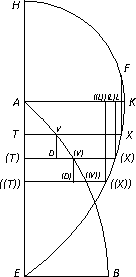
\includegraphics[width=0.35\textwidth]{gesamttex/edit_VIII,3/images/LH_37_05_045-046_d1.pdf}}%
  \vspace{0.5em}
  \centerline{\lbrack\textit{Fig.~1}\rbrack}%
  \label{LH_37_05_045r_d1_Fig.1}%
%  \vspace{1.0em}%
  %\newpage%
%
%
\newpage
\count\Bfootins=1000
\count\Afootins=1200
\count\Cfootins=1000
\pstart
\noindent 
\lbrack\textit{(V)(T)((T))}\rbrack.
%
Seu incrementa areae \textit{ATV}%
\protect\index{Sachverzeichnis}{incrementum areae}
fore proportionalia%
\protect\index{Sachverzeichnis}{incrementum proportionale}
incrementis tensionum depositarum \textit{KL},%
\protect\index{Sachverzeichnis}{incrementum tensionis depositae}%
\protect\index{Sachverzeichnis}{tensio deposita}
seu ipsas areas \textit{ATV} fore
tensionibus depositis \textit{KL}%
\protect\index{Sachverzeichnis}{tensio deposita}
%\edlabel{LH_37_05_045-046_m045r5}%
proportionales.%
\pend%
%
%
\pstart%
Jam%
\edlabel{LH_37_05_045-046_m045r4}
%\edlabel{LH_37_05_045-046_m045r6}
sumamus aliquam legem\protect\index{Sachverzeichnis}{lex solicitationis}
%
\edtext{solicitationis.%
\protect\index{Sachverzeichnis}{solicitatio decrescens}
Et quoniam manifestum est,
solicitationem cum tensione superstite%
\protect\index{Sachverzeichnis}{tensio superstes}
decrescere%
\protect\index{Sachverzeichnis}{solicitatio decrescens}%
\protect\index{Sachverzeichnis}{tensio decrescens}
ac denique desinere%
\protect\index{Sachverzeichnis}{solicitatio desinens}%
\protect\index{Sachverzeichnis}{tensio desinens}%
\lbrack,\rbrack\
fingamus
solicitationes\protect\index{Sachverzeichnis}{solicitatio tensioni proportionalis}
esse}{%
\lemma{solicitationis}\Bfootnote{%
\textit{(1)}~, et fingamus si placet,
\textit{(a)}~tensiones esse
\textit{(b)}~solicitationes esse
\textit{(2)}~. Et quoniam manifestum est,
\textit{(a)}~decrescente
\textit{(b)}~solicitationem cum tensione
\textbar~superstite \textit{erg.}~%
\textbar\ decrescere ac % denique desinere fingamus 
\lbrack...\rbrack\ solicitationes esse%
~\textit{L}}}
%
tensionibus residuis proportionales;%
\protect\index{Sachverzeichnis}{tensio solicitationi proportionalis}%
\protect\index{Sachverzeichnis}{tensio residua}
seu esse \textit{D(V)} ad \textit{(D)((V))}
$\stackrel{(2)}{\text{ut}}$
\textit{AL} ad \textit{A(L)}.%
\pend%
% \newpage%
%
\pstart%
Ob artic.~1,%
\protect\index{Sachverzeichnis}{articulus}
$T\textit{(T)}\cdot TV:L\textit{(L)}$ $\stackrel{(3)}{\text{est}}$
quantitas constans%
\protect\index{Sachverzeichnis}{quantitas constans}
%
\edtext{velocitatem quandam repraesentans%
\protect\index{Sachverzeichnis}{quantitas velocitatem repraesentans}%
}{%
\lemma{velocitatem}\Bfootnote{%
\hspace{-0,5mm}quandam repraesentans
\textit{erg.~L}}}
%
quam vocemus \textit{b}.
Et fiet $T\textit{(T)}\cdot TV\stackrel{(4)}{=}b\cdot L\textit{(L)}.$%
\pend%
%
\pstart%
Ob
\edtext{artic.~2,%
\protect\index{Sachverzeichnis}{articulus}
$DV:AL$}{%
{\lemma{artic. 2,}\Bfootnote{\hspace{-0,5mm}%
\textbar~est \textit{streicht Hrsg.}~%
\textbar\ $DV:AL$%
~\textit{L}}}%
{\lemma{\textit{DV}}\Cfootnote{%
Gemeint ist stattdessen das Differentiaelement \textit{D(V)}, die \textit{solicitatio}.
Der Fehler wiederholt sich ausnahmslos bis zu S.~\refpassage{LH_37_05_045v_errorDV}{LH_37_05_045v_errorDV},
ohne aber das Ergebnis der Gesamtrechnung zu verfälschen,
und wird demgemäß vom Herausgeber nicht berichtigt.%
}}}
%
$\stackrel{(5)}{\text{est}}$
quantitas constans,%
\protect\index{Sachverzeichnis}{quantitas constans}
%
\edtext{sed hinc sequitur%
\lbrack,\rbrack\
quemadmodum et ex artic.~2,%
\protect\index{Sachverzeichnis}{articulus}
ut temporis%
\protect\index{Sachverzeichnis}{tempus restitutionis}
et spatii%
\protect\index{Sachverzeichnis}{spatium restitutionis}
progressus%
\protect\index{Sachverzeichnis}{progressus temporis}%
\protect\index{Sachverzeichnis}{progressus spatii}
talis assignari non possit,
qui velocitates uniformiter crescere%
\protect\index{Sachverzeichnis}{velocitas uniformiter crescens}
faciat;}{%
\lemma{sed}\Bfootnote{%
\textit{(1)}~hinc sequitur
\textit{(2)}~hinc
\textit{(a)}~sequi videtur absurdum, ut scilicet velocitatum incrementa
\textit{(b)}~sequitur quemadmodum et ex artic.~2,
\textit{(aa)}~ut scilicet velocitatum incrementa u
\textit{(bb)}~ut velocitates
\textit{(cc)}~ut temporis
\textit{(aaa)}~vel
\textit{(bbb)}~et spatii % progressus talis assignari non 
\lbrack...\rbrack\ possit, qui
\textit{(aaaa)}~et
\textit{(bbbb)}~velocitates uniformiter crescere faciat;%
~\textit{L}}}
%
nam alioqui etiam \textit{AL} foret constans,
si \textit{DV} fieret
%
\edtext{constans.%
\protect\index{Sachverzeichnis}{quantitas constans}
Sed absurdum%
\protect\index{Sachverzeichnis}{absurdum}
omnino est non posse ipsas \textit{TV},
ordinatas curvae \textit{V(V)},%
\protect\index{Sachverzeichnis}{curva}
assumi uniformiter crescentes.%
\protect\index{Sachverzeichnis}{velocitas uniformiter crescens}%
}{%
\lemma{constans.}\Bfootnote{%
\textit{(1)}~Quod probe notandum est, assumamus \textit{T(T)} $\stackrel{(6)}{\text{esse}}$ constantem; hoc enim semper possibile est,
\textit{(2)}~Sed
\textit{(a)}~hoc ipsum videtur
\textit{(b)}~absurdum omnino
\textit{(aa)}~, ut
\textit{(bb)}~est
\textit{(aaa)}~ipsarum ordinatarum
\textit{(bbb)}~ut re
\textit{(ccc)}~ut
\textit{(ddd)}~non posse % ipsas \textit{TV}, ordinatas curvae \textit{V(V)}, assumi 
\lbrack...\rbrack\ uniformiter crescentes.%
~\textit{L}}}
%
Itaque hinc colligitur
$\stackrel{(6)}{\text{impossibilem}}$
esse articulum (2)%
\protect\index{Sachverzeichnis}{articulus}
%
\edtext{absolute sumtum%
\lbrack,\rbrack%
}{%
\lemma{absolute}\Bfootnote{%
\hspace{-0,5mm}sumtum
\textit{erg.~L}}}
%
ut tensiones sint elementis velocitatum%
\protect\index{Sachverzeichnis}{tensio velocitati proportionalis}%
\protect\index{Sachverzeichnis}{elementum velocitatis}
%
\edtext{proportionales.
Imo}{%
\lemma{proportionales.}\Bfootnote{%
\textit{(1)}~Sed
\textit{(2)}~Imo%
~\textit{L}}}
%
generaliter impossibilis est hypothesis%
\protect\index{Sachverzeichnis}{hypothesis}%
\lbrack:\rbrack\
elementis rei continue crescentis aut%
\protect\index{Sachverzeichnis}{elementum rei continue crescentis}%
\protect\index{Sachverzeichnis}{res continue crescens}
%
\edtext{decrescentis,%
\protect\index{Sachverzeichnis}{elementum rei continue decrescentis}%
\protect\index{Sachverzeichnis}{res continue decrescens}
res alias continue proportionales%
\protect\index{Sachverzeichnis}{res continue proportionalis}
facere.
Ergo articuli 2 et 5 tantum habent locum,}{%
\lemma{decrescentis,}\Bfootnote{%
\textit{(1)}~rem ind
\textit{(2)}~rem
\textit{(3)}~res alias continue
\textit{(a)}~\textbar~crescentes \textit{streicht Hrsg.}~%
\textbar\ aut decrescen
\textit{(b)}~proportionales facere.
\textit{(aa)}~Ergo loco artic.
\textit{(bb)}~Ergo articuli % 2 et 5 tantum 
\lbrack...\rbrack\ habent locum,%
~\textit{L}}}
%
si dicamus
ipsas \textit{DV} esse in ratione composita%
\lbrack,\rbrack\
ipsarum \textit{AL}
%
\edtext{directa,}{%
\lemma{directa}\Bfootnote{%
\textit{erg.~L}}}
%
et aliorum
%
\edtext{quorundam}{%
\lemma{quorundam}\Bfootnote{%
\textit{erg.~L}}}
%
elementorum
%
\edtext{$d\omega$ reciproca}{%
\lemma{$d\omega$}\Bfootnote{%
\hspace{-0,5mm}reciproca
\textit{erg.~L}}}
%
quae si constantia assumantur,%
\protect\index{Sachverzeichnis}{elementum constans}
seu esse \textit{DV}
$\stackrel{(7)}{\text{ut}}$ $AL\,d\omega,$
ita tum demum
cum $d\omega$ est constans
locum
%
\edtext{\lbrack habebunt\rbrack}{%
\lemma{habebit}\Bfootnote{%
\textit{L~ändert Hrsg.}}}
%
artic.~2 et~5.%
\protect\index{Sachverzeichnis}{articulus}
Et non licuisset facere
\textit{DV}, $d\omega$ ut \textit{AL},
nam et sic elementare esset ordinario proportionale,%
\protect\index{Sachverzeichnis}{elementare ordinario proportionale}
sed $DV:d\omega,$
id enim constans%
\protect\index{Sachverzeichnis}{elementum constans}
assumi in arbitrio non est.%
\protect\index{Sachverzeichnis}{arbitrium}
Faciamus ergo
%
%\edtext{ $DV=ALd\omega :f.$}{%
%\lemma{ergo}\Bfootnote{%
%\textit{(1)}~$DV=ALd\omega :f$
%\textit{(2)}~$DV=ALd\omega :f.$%
%~\textit{L}}}
%
\lbrack45~v\textsuperscript{o}\rbrack\    %%%%    Blatt 45v
%
%\pend%
%%
%\pstart%
$DV\stackrel{(8)}{=}AL\,d\omega :f.$%
\edlabel{LH_37_05_045v_errorDV}
\pend%
%\newpage%
%
\pstart%
Nunc ut calculum absolvamus%
\protect\index{Sachverzeichnis}{calculus absolvendus}%
\lbrack:\rbrack\
\textit{AL} sit \textit{x}
%
\edtext{et \textit{L(L)} erit \textit{dx},}{%
\lemma{et}\Bfootnote{%
\hspace{-0,5mm}\textit{L(L)} erit \textit{dx}
\textit{erg.~L}}}
%
et \textit{TV} sit \textit{v}
et \textit{D(V)} erit \textit{dv},
et \textit{AT} sit \textit{t}
et \textit{T(T)} erit \textit{dt}.
%\pend%
%\newpage%
%%
%\pstart%
His positis%
\lbrack,\rbrack\
ex artic.~4
%
\edtext{fiet
\edtext{$v\,dt\stackrel{(8)}{=}b\,dx.$}{%
\lemma{$v\,dt\stackrel{(8)}{=}b\,dx$}\Cfootnote{%
Gemäß der bisherigen Nummerierung sollte das die Gleichung ((8)) sein.}}%
}{%
\lemma{fiet}\Bfootnote{%\hspace{-0,5mm}
\textit{(1)}~\textit{dt}
\textit{(2)}~$v=$
\textit{(a)}~\textit{dt}
\textit{(b)}~\textit{b}
\textit{(3)}~$v\,dt\stackrel{(8)}{=}b\,dx.$%
~\textit{L}}}
%
Et ex artic.~8
fiet
$dv\stackrel{(9)}{=}x\,d\omega:f.$
Si fingeremus esse
$dt\stackrel{((9))}{=}d\omega,$
fieret
\edlabel{LH_37_05_045v_Gleichung10-1}%
$b\,dx:v\stackrel{(10)}{=}f\,dv:x,$%
\edlabel{LH_37_05_045v_Gleichung10-2}
seu $bx\,dx \stackrel{(11)}{=}
%
\edtext{fv\,dv,$
seu
$bxx \stackrel{(12)}{=} \edtext{fhh-vv,$}{%
\lemma{$fhh-vv$}\Cfootnote{%
Zu lesen wie: $f(h^2 - v^2).$}}
quia scilicet crescentibus \textit{v}
decrescent \textit{x},
et cum \textit{x} seu \textit{AL} evanescit%
\protect\index{Sachverzeichnis}{quantitas evanescens}
seu \textit{v} est maxima,
fit}{%
\lemma{\textit{fv\,dv}}\Bfootnote{%
\textit{(1)}~\textbar~et quia \textit{streicht Hrsg.}~\textbar\
\textit{(a)}~cresc
\textit{(b)}~\textit{x} evan
\textit{(2)}~seu \textit{bxx} % $\stackrel{(12)}{=}fhh-vv,$ quia scilicet crescentibus \textit{v} decrescent \textit{x}, et cum \textit{x} seu 
\lbrack...\rbrack\ \textit{AL} evanescit
\textbar~seu \textit{v} est maxima \textit{erg.}~%
\textbar~, fit%
~\textit{L}}}
%
$0\stackrel{(13)}{=}hh-vv.$
%
\edtext{Ergo \textit{h} erit velocitas maxima.%
\protect\index{Sachverzeichnis}{velocitas maxima}}{%
\lemma{Ergo \lbrack...\rbrack\ maxima}\Cfootnote{%
Später
(S.~\refpassage{LH_37_05_045v_h=AK-1}{LH_37_05_045v_h=AK-2}; \refpassage{LH_37_05_045v_AK=tensiomaxima-1}{LH_37_05_045v_AK=tensiomaxima-2})
wird \textit{h} indessen mit \textit{AH} bzw. \textit{AK} gleichgesetzt,
d.h. mit der größten Spannkraft.%
}}
%
Hinc fiet
$v\stackrel{(14)}{=}\sqrt{hh-\displaystyle\frac{b}{f}xx}.$
Eritque
$dt\stackrel{(15)}{=}b\,dx:
%
\edtext{}{%
{\xxref{LH_37_05_045-046_m045v1}{LH_37_05_045-046_m045v2}}%
{\lemma{$\sqrt{hh-\overline{b:f}xx}$}\Bfootnote{%
\textit{(1)}~. Faciemus \textit{b} et \textit{h} et \textit{f} aequales, id enim in nostra potestate est, et fiet $dt \stackrel{(16)}{=} b\,dx:\sqrt{bb-xx},$
\textit{(a)}~\textit{b} existente
\textit{(b)}~ponendo scil.
\textit{(aa)}~$AK=AE=h$
\textit{(bb)}~\textit{AK} seu $h=AE$ seu \textit{b}. His ita positis si centro \textit{A} radio
\textit{(aaa)}~\textit{AH}
\textit{(bbb)}~\textit{AK}
\textit{(ccc)}~\textit{AK} vel \textit{EB} describatur quadrans \textit{HFK} cui
\textit{(aaaa)}~per \textit{L} ducta \textit{AK}
\textit{(bbbb)}~ex \textit{AL} normaliter educta \textit{LF} occurrat in \textit{F} multipli
\textit{(2)}~, seu $dt \stackrel{(16)}{=}$
\textit{(a)}~$b\sqrt{b:f}:$
\textit{(b)}~$\displaystyle\frac{b}{\sqrt{b:f}}\displaystyle\frac{dx}{\displaystyle\sqrt{\frac{hh}{b:f}-xx}}.$ Fiat $b \stackrel{(17)}{=} f,$
\textbar~seu $dv \stackrel{((17))}{=} x\,dt$ :
\textbar~\textit{f} \textit{ändert Hrsg.}~%
\textbar~, \textit{erg.}~%
\textbar\ id enim % cum eas pro arbitrio assumserimus, et assumere potuerimus, in potestate est, et fiet $dt \stackrel{(18)}{=} b\,dx:\sqrt{hh-xx}.$ Sit $b \stackrel{(19)}{=} 7h$ (\protect\vphantom)sumto 7 pro numero quocunque et fiet 
\lbrack...\rbrack\ $h\,dt \stackrel{(20)}{=} bh\,dx:\sqrt{hh-xx}.$
\textit{(aa)}~Centro
\textit{(bb)}~Jam centro \textit{A} radio \textit{AK} describatur
\textit{(aaa)}~circulus
\textit{(bbb)}~quadrans circularis % \textit{KFH}, et ex \textit{AL} 
\lbrack...\rbrack\ seu \textit{x}
\textit{(aaaa)}~erigatur \textit{LF}
\textit{(bbbb)}~normaliter educatur \textit{LF},%
~\textit{L}}}}%
%
\edlabel{LH_37_05_045-046_m045v1}%
\sqrt{hh-\overline{b:f}\;xx},$
seu
$dt \stackrel{(16)}{=} \displaystyle\frac{b}{\sqrt{b:f}}\displaystyle\frac{dx}{\displaystyle\sqrt{\frac{hh}{b:f}-xx}}.$
Fiat $b \stackrel{(17)}{=} f,$
seu $dv \stackrel{((17))}{=} x\,dt:[b],$ % f
id enim cum eas pro arbitrio assumserimus%
\protect\index{Sachverzeichnis}{arbitrium} % ,
et assumere potuerimus,
in potestate est,%
\protect\index{Sachverzeichnis}{potestas}
et fiet $dt \stackrel{(18)}{=} b\,dx:\sqrt{hh-xx}.$
Sit $b \stackrel{(19)}{=} 7h$
(\protect\vphantom)%
sumto 7 pro numero quocunque%
\lbrack\protect\vphantom()\rbrack\
et fiet
$h\,dt \stackrel{(20)}{=} bh\,dx:\sqrt{hh-xx}.$%
\pend%
%
%
%  \newpage% 
  \vspace{1.5em}%	% Diagramm Fig.~2
  \centerline{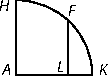
\includegraphics[width=0.18\textwidth]{gesamttex/edit_VIII,3/images/LH_37_05_045-046_d2.pdf}}%
  \vspace{0.5em}
  \centerline{\lbrack\textit{Fig.~2}\rbrack}%
  \label{LH_37_05_045v_Fig.2}%
 % \vspace{1.05em}%
 \newpage%
%
%
\pstart%
Jam centro \textit{A} radio \textit{AK}%
\protect\index{Sachverzeichnis}{radius}
describatur quadrans circularis \textit{KFH},%
\protect\index{Sachverzeichnis}{quadrans circularis}
et ex \textit{AL} seu \textit{x} normaliter educatur \textit{LF},%
\edlabel{LH_37_05_045-046_m045v2}
%
erit
$\displaystyle h\!\!\int\!\overline{dx:\sqrt{hh-xx}}\stackrel{(21)}{=}\text{arc.}\;KF,$
et in casu \textit{L} incidentis in \textit{A}
seu \textit{x} evanescentis,%
\protect\index{Sachverzeichnis}{quantitas evanescens}
erit
$\displaystyle h\!\!\int\!\overline{dx:\sqrt{hh-xx}} \stackrel{(22)}{=} \text{arcus}$ quadrant.%
\protect\index{Sachverzeichnis}{arcus quadrantis}
%
\edtext{\textit{KFH}.
Sed
\edtext{$\displaystyle ht \stackrel{(22)}{=} bh\!\!\int\!\overline{dx:\sqrt{hh-xx}}.$}{%
\lemma{$\displaystyle ht \stackrel{(22)}{=} bh\!\!\int\!\overline{dx:\sqrt{hh-xx}}.$}\Cfootnote{%
Gemäß der bisherigen Nummerierung sollte das die Gleichung ((22)) sein.}}
Ergo \textit{t} seu tempus \textit{AT}%
\protect\index{Sachverzeichnis}{tempus restitutionis}
est ad \textit{b} constantem assumtam,
$\displaystyle\stackrel{(23)}{\text{ut}} h\!\!\int\!\overline{dx:\sqrt{hh-xx}}$
seu arcus \textit{KF}
est ad
\edlabel{LH_37_05_045v_h=AK-1}%
\textit{h} seu radium \textit{AK}.%
\edlabel{LH_37_05_045v_h=AK-2}
Et in casu totius temporis \textit{AE},
totum tempus \textit{AE}%
\protect\index{Sachverzeichnis}{tempus restitutionis}
est ad \textit{b} constantem assumtam,
$\stackrel{(24)}{\text{ut}}$ arcus quadrantis \textit{KFH}%
\protect\index{Sachverzeichnis}{arcus quadrantis}
est ad radium \textit{AH},%
\protect\index{Sachverzeichnis}{radius}
quae ratio cum sit constans,%
\protect\index{Sachverzeichnis}{ratio constans}
etiam sequitur tempus constans esse,%
\protect\index{Sachverzeichnis}{tempus constans}%
\protect\index{Sachverzeichnis}{isochronismus restitutionis}%
}{%
\lemma{\textit{KFH}.}\Bfootnote{%
\textit{(1)}~Ergo fit $dt=t$
\textit{(2)}~Sed $\displaystyle ht \stackrel{(22)}{=} bh\!\!\int\!\overline{dx:\sqrt{hh-xx}}.$
\textit{(a)}~Ergo
\textit{(aa)}~$t=KF$
\textit{(bb)}~$t=KF$
\textit{(cc)}~$t:b$
\textit{(dd)}~tandem
\textit{(b)}~Ergo fit tandem in casu totius temporis $t:b \stackrel{(23)}{=} KFH:AK$ seu \textit{h}, id est tempus \textit{t}
\textbar~totum \textit{erg.}~%
\textbar\ est ad constantem \textit{b}, ut arcus quadrantis ad radium.
Itaque tempus
\textit{(aa)}~ipsum
\textit{(bb)}~totum ipsummet est constans. Ergo $\displaystyle t:b \stackrel{(23)}{=} h\!\!\int\!\overline{dx:\sqrt{hh-xx}},$ seu $KFH:h$ seu \textit{AK}, id est tempus \textit{t}
\textit{(c)}~Ergo \textit{t} seu % tempus \textit{AT} est ad \textit{b} constantem 
\lbrack...\rbrack\ assumtam $\stackrel{(23)}{\text{ut}}$
\textbar~ ut \textit{streicht Hrsg.}~%
\textbar\ $\displaystyle h\!\!\int\!\overline{dx:\sqrt{hh-xx}}$ seu % ... 
\lbrack...\rbrack\ tempus constans esse,%
~\textit{L}}}
%
nec referre,
quanta sit
\edlabel{LH_37_05_045v_AK=tensiomaxima-1}%
maxima tensio%
\protect\index{Sachverzeichnis}{tensio maxima}
%
\edtext{\textit{AK},%
\edlabel{LH_37_05_045v_AK=tensiomaxima-2}%
}{%
\lemma{\textit{AK}}\Bfootnote{%
\textit{erg.~L}}}
%
adeoque et
%
\edtext{solicitatio ab ea}{%
\lemma{solicitatio}\Bfootnote{\hspace{-0,5mm}%
\textbar~\textit{AK} \textit{gestr.}~%
\textbar\ ab
\textit{(1)}~eam
\textit{(2)}~ea%
~\textit{L}}}
%
dependens.%
\protect\index{Sachverzeichnis}{solicitatio a tensione dependens}%
\pend%
%
\pstart%
Hoc autem
quod finxisse visi sumus
verissimum est,
si scilicet tensionibus proportionales sunt%
\protect\index{Sachverzeichnis}{tensio solicitationi proportionalis}
%
\edtext{\lbrack solicitationes\rbrack,%
\protect\index{Sachverzeichnis}{solicitatio}%
}{%
\lemma{solitationes}\Bfootnote{%
\textit{L~ändert Hrsg.}}}
%
id intelligendum esse
aequalibus temporis elementis.%
\protect\index{Sachverzeichnis}{elementa temporis aequalia}
%
\edtext{Nam longiore tempore%
\protect\index{Sachverzeichnis}{tempus restitutionis}
eadem tensio vel parum diversa
(\protect\vphantom)%
pro quibus media sumi potest%
\protect\vphantom()%
}{%
\lemma{Nam}\Bfootnote{%
\textit{(1)}~eadem
\textit{(2)}~longiore tempore eadem tensio
\textit{(a)}~\textbar~vel \textit{streicht Hrsg.}~%
\textbar\ certe ae
\textit{(b)}~vel parum diversa
\textbar~(\protect\vphantom)pro quibus media sumi potest\protect\vphantom()
\textit{erg.~L}}}
%
diutius solicitans,%
\protect\index{Sachverzeichnis}{tensio solicitans}
majorem etiam imprimet conatum.%
\protect\index{Sachverzeichnis}{conatus tensione impressus}
Nec quicquam momento productum intelligi potest.%
\protect\index{Sachverzeichnis}{momentum temporis}%
\protect\index{Sachverzeichnis}{productum momento}%
\pend%
%
\pstart%
Sed hoc amplius videtur ostendi posse,
etiamsi non
%
\edtext{sint impressiones%
\protect\index{Sachverzeichnis}{impressio tensioni proportionalis}
aequalibus tempusculis factae,%
\protect\index{Sachverzeichnis}{tempuscula aequalia}
tensionibus proportionales,%
\protect\index{Sachverzeichnis}{tensio impressioni proportionalis}%
}{%
\lemma{sint}\Bfootnote{%
\textit{(1)}~solicit
\textit{(2)}~impressiones
\textit{(a)}~temp
\textit{(b)}~tensionibus
\textit{(c)}~aequalibus
\textit{(aa)}~tempusculis factae
\textit{(bb)}~tempusculis factae,
\textit{(aaa)}~tem
\textit{(bbb)}~tensionibus
\textit{(aaaa)}~prop
\textit{(bbbb)}~proportionales,%
~\textit{L}}}
%
sed utcunque ex ipsis et maxima tensione%
\protect\index{Sachverzeichnis}{tensio maxima}
%
\edtext{pendeant,
obtineri}{%
\lemma{pendeant,}\Bfootnote{%
\textit{(1)}~seu utcunque
\textit{(a)}~\textit{dv} definiatur
\textit{(b)}~$dv:d\omega$ definiatur ex recta
\textit{(2)}~videri
\textit{(3)}~obtineri%
~\textit{L}}}
%
isochronismum.%
\protect\index{Sachverzeichnis}{isochronismus restitutionis}
Nempe scribatur:
pro $d\omega$ ponamus \textit{dt}
per ((9)),
et pro \textit{x} in aeq.~9%
\protect\index{Sachverzeichnis}{aequatio}
ponatur recta \textit{\~x}
determinata utcunque per homogeneas \textit{x} et \textit{h},%
\protect\index{Sachverzeichnis}{quantitas homogenea}
%
\edtext{fiet $dv:dt \stackrel{(25)}{=} \tilde{x}:f.$}{%
\lemma{fiet}\Bfootnote{%
\textit{(1)}~$dv=\tilde{x}:$
\textit{(2)}~$dv:dt\stackrel{(25)}{=}\tilde{x}:f.$%
~\textit{L}}}
%
Et per 11 et 8,
fiet $v\,dv \stackrel{(26)}{=} \overline{b:f}\;\tilde{x}\,dx,$
seu
$\displaystyle \frac{1}{2}vv \stackrel{(27)}{=} \overline{b:f}\!\!\int\!\overline{\tilde{x}\,dx},$
seu posita  $b=f$ per
\pend
\newpage
\pstart
\noindent 17,
fiet
$\displaystyle \frac{1}{2}vv \stackrel{(28)}{=} \!\!\int\!\overline{\tilde{x}\,dx},$
seu
$\displaystyle v \stackrel{(29)}{=} \sqrt{2}\sqrt{\!\!\int\!\overline{\tilde{x}\,dx}}.$
Et per 8
%
%\edtext{}{%
%\lemma{per 8}\Cfootnote{%
%Gemeint ist wohl eher die Gleichung 10, S.~\refpassage{LH_37_05_045v_Gleichung10-1}{LH_37_05_045v_Gleichung10-2}.???
%}}
%
fiet
$\displaystyle dt \stackrel{(30)}{=} b\,dx : \sqrt{2\!\!\int\!\overline{\tilde{x}\,dx}}.$
Porro in
%
\edtext{casu maximi temporis,%
\protect\index{Sachverzeichnis}{casus}%
\protect\index{Sachverzeichnis}{tempus maximum}
quo \textit{x} evanescit,%
\protect\index{Sachverzeichnis}{quantitas evanescens}
debet \textit{\~x}
(\protect\vphantom)%
quippe ex solis%
}{%
\lemma{casu}\Bfootnote{%
\textit{(1)}~quo \textit{x}
\textit{(2)}~maximi temporis, quo
\textit{(a)}~\textit{h} eva
\textit{(b)}~\textit{x} evanescit,
\textit{(aa)}~potest
\textit{(bb)}~debet \textit{\~x}
\textit{(aaa)}~ex solis
\textit{(bbb)}~(\protect\vphantom{)}quippe ex solis%
~\textit{L}}}
%
\textit{x} et \textit{h} generaliter,
adeoque nunc ex sola \textit{h} determinata% ,
\lbrack\protect\vphantom()\rbrack\
necessario coincidere cum \textit{h}
multiplicata per numerum constantem%
\protect\index{Sachverzeichnis}{numerus constans}
seu determinatam rationem.%
\protect\index{Sachverzeichnis}{ratio determinata}
Ergo eodem casu
$\displaystyle \!\!\int\!\overline{\tilde{x}\,dx}$
necessario est \textit{hh}
multiplicata per numerum constantem.
%
Ergo
$\displaystyle\sqrt{\!\!\int\!\overline{\tilde{x}\,dx}}$
utique
%\edtext{}{%
%\lemma{Ergo}\Bfootnote{%
%\textit{(1)}~$\surd\int\tilde{x}dx$
%\textit{(2)}~$\int\overline{\tilde{x}dx}$
%\textit{(a)}~necessari
%\textit{(b)}~utique%
%~\textit{L}}}
%
est \textit{h} multiplicata per numerum constantem.%
\protect\index{Sachverzeichnis}{numerus constans}
Et
$\displaystyle t:b \stackrel{(31)}{=} \!\!\int\!\overline{dx:\sqrt{2\!\!\int\!\overline{\tilde{x}\,dx}}}.$
%
Ubique hoc eodem casu,
quo \textit{x} evanescit,
%
\edtext{est ratio constans,%
\protect\index{Sachverzeichnis}{ratio constans}%
}{%
\lemma{est}\Bfootnote{%
\textit{(1)}~numerus constans
\textit{(2)}~ratio constans,%
~\textit{L}}}
%
evanescente \textit{h},%
\protect\index{Sachverzeichnis}{quantitas evanescens}
cum a parte dextra aequationis 31%
\protect\index{Sachverzeichnis}{aequatio}
non nisi una homogenea,
nempe \textit{h},%
\protect\index{Sachverzeichnis}{quantitas homogenea}
occurrere possit,
quae proinde,
ubi res ad rationem redit%
\protect\index{Sachverzeichnis}{res ad rationem reddita} % ,
seu analogiam inter%
\protect\index{Sachverzeichnis}{analogia inter homogenea}
%
%\edlabel{LH_37_05_045-046_m045v3}%
\edtext{homogenea,
sed hoc loco
%
\lbrack46~r\textsuperscript{o}\rbrack\  %%%% Blatt 46r
%
ejusdem ad semet}{%
\lemma{homogenea,}\Bfootnote{%
\textit{(1)}~id est idem ad sem
\textit{(2)}~sed hoc loco \lbrack46~r\textsuperscript{o}\rbrack\ ejusdem
\textit{(a)}~sem
\textit{(b)}~ad semet%
~\textit{L}}}
%
rationem%
\protect\index{Sachverzeichnis}{ratio ejusdem ad semet}
%\edlabel{LH_37_05_045-046_m045v4}
cum numerica ratione compositam%
\lbrack,\rbrack\
necessario evanescit,
sola ratione numerica manente,
%
\edtext{adeoque tempus est%
\protect\index{Sachverzeichnis}{tempus restitutionis}%
}{%
\lemma{adeoque}\Bfootnote{%
\textit{(1)}~est
\textit{(2)}~tempus est%
~\textit{L}}}
%
constans%
\protect\index{Sachverzeichnis}{tempus constans}
seu idem%
\protect\index{Sachverzeichnis}{isochronismus restitutionis}%
\lbrack,\rbrack\
quaecunque demum sumatur \textit{h}
seu tensio elastri ejusdem.%
\protect\index{Sachverzeichnis}{tensio elastri}%
\pend%
%
\pstart%
Hoc etiam ocularius % ,
et magis
%
\edtext{ad captum%
\protect\index{Sachverzeichnis}{captus}%
}{%
\lemma{ad}\Bfootnote{\hspace{-0,5mm}%
\textbar~vulgi \textit{gestr.}~%
\textbar~captum%
~\textit{L}}}
%
ex
%
\edtext{\lbrack serie\rbrack}{%
\lemma{seriei}\Bfootnote{%
\textit{L~ändert Hrsg.}}}
%
infinita%
\protect\index{Sachverzeichnis}{series infinita}
educi potest,
%
nam generalissime
%\edtext{}{%
%\lemma{nam}\Bfootnote{%
%\textit{(1)}~ne
%\textit{(2)}~generalissime%
%~\textit{L}}}
%
$t:b\stackrel{(32)}{=}10+11\displaystyle\frac{x}{h}+12\displaystyle\frac{xx}{hh}+13\displaystyle\frac{x^3}{h^3},$%
\rule[-4mm]{0pt}{10mm}
%
\edtext{etc.
ubi 10, 11, 12 sunt numeri%
\protect\index{Sachverzeichnis}{numerus constans}
seu rationes constantes,%
\protect\index{Sachverzeichnis}{ratio constans}
neque}{%
\lemma{etc.}\Bfootnote{\hspace{-0,5mm}%
\textbar~ubi 10, % 11, 12 sunt numeri seu 
\lbrack....\rbrack\ rationes constantes,
\textbar~homogeneae
\textit{gestr.}~\textbar\
\textit{erg.}~\textbar\ neque%
~\textit{L}}}
%
possibile est % ,
ut aliter
%
\edtext{exprimatur,
cum ratio \textit{t} ad \textit{b}%
}{%
\lemma{exprimatur,}\Bfootnote{%
\textit{(1)}~cum determinetur ex ratione \textit{x} a
\textit{(2)}~cum ratio \textit{t} ad \textit{b}%
~\textit{L}}}
%
per solas \textit{x} et \textit{h} determinetur
%
\edtext{\lbrack in\rbrack}{%
\lemma{in}\Bfootnote{%
\textit{rg. Hrsg.}}}
%
aeq.~31.%
\protect\index{Sachverzeichnis}{aequatio}
Ergo non nisi per $x:h,$
nec vero adhiberi potest $h:x,$
%
\edtext{quia evanescente \textit{x},%
\protect\index{Sachverzeichnis}{quantitas evanescens}
seu in casu maximi temporis%
\protect\index{Sachverzeichnis}{tempus maximum}
foret talis terminus}{%
\lemma{quia}\Bfootnote{%
\textit{(1)}~terminus qu
\textit{(2)}~evanescente \textit{x}, seu in casu
\textit{(a)}~maximae tensionis, seu
\textit{(b)}~maximi temporis foret talis terminus%
~\textit{L}}}
%
infinitus.%
\protect\index{Sachverzeichnis}{terminus infinitus}
At vero in casu maximi temporis%
\protect\index{Sachverzeichnis}{casus}%
\protect\index{Sachverzeichnis}{tempus maximum}
seu ubi $x = 0$ evanescentibus omnibus,%
\protect\index{Sachverzeichnis}{quantitas evanescens}
$t : b$ $\stackrel{(33)}{\text{aequatur}}$
numero constanti 10.%
\protect\index{Sachverzeichnis}{numerus constans}
%
\edtext{Et exemplo%
\protect\index{Sachverzeichnis}{exemplum}
assumtae qualiscunque solicitationum legis%
\protect\index{Sachverzeichnis}{lex solicitationis}
res evinci potest.
Ut si solicitationes%
\protect\index{Sachverzeichnis}{solicitatio ut quadratum tensionis}
sint ut quadrata tensionum,%
\protect\index{Sachverzeichnis}{quadratum tensionis}%
\protect\index{Sachverzeichnis}{tensio elastri}
seu \textit{dv} ut \textit{xx\,dt},
idem comperietur.%
}{%
\lemma{Et}\Bfootnote{%
\hspace{-0,5mm}exemplo assumtae qualiscunque
\textit{(1)}~regulae
\textit{(2)}~solicitationum legis % res evinci potest. Ut si solicitationes sint ut quadrata 
\lbrack...\rbrack\ tensionum, seu
\textit{(a)}~ut
\textit{(b)}~\textit{dv} ut \textit{xx\,dt}, idem comperietur.
\textit{erg.~L}}}%
\pend%
%
\pstart%
His ita%
\edlabel{LH_37_05_046r_Isochronismusbeweis-1}
%
\edtext{tandem mirabilis naturae arcani%
\protect\index{Sachverzeichnis}{arcanum naturae}%
}{%
\lemma{tandem}\Bfootnote{%
\textit{(1)}~ho
\textit{(2)}~arcana
\textit{(3)}~mirabilis naturae arcani%
~\textit{L}}}
%
rationem reddidimus.
Sensu%
\protect\index{Sachverzeichnis}{sensus}
enim
%
\edtext{deprehenditur
aequales esse sonos%
\protect\index{Sachverzeichnis}{sonus aequalis}
adeoque et vibrationes%
\protect\index{Sachverzeichnis}{vibratio aequalis}%
\protect\index{Sachverzeichnis}{isochronismus vibrationis}
vel restitutiones,%
\protect\index{Sachverzeichnis}{restitutio aequalis}%
\protect\index{Sachverzeichnis}{isochronismus restitutionis}
sive fortiter sive mollius rem tensam pulsemus.%
\protect\index{Sachverzeichnis}{pulsatio fortis}%
\protect\index{Sachverzeichnis}{pulsatio mollis}%
\protect\index{Sachverzeichnis}{res pulsata}%
\protect\index{Sachverzeichnis}{res tensa}%
}{%
\lemma{deprehenditur}\Bfootnote{%
\textit{(1)}~tensi
\textit{(2)}~tensionum ve
\textit{(3)}~aequales esse % sonos adeoque et vibrationes vel restitutiones, sive fortiter sive mollius rem 
\lbrack...\rbrack\ tensam pulsemus.%
~\textit{L}}}
%
Itaque
%
\edtext{licet quamcunque legem%
\protect\index{Sachverzeichnis}{lex conatuum}
conatus}{%
\lemma{licet}\Bfootnote{%
\textit{(1)}~conatus
\textit{(2)}~conatus
\textit{(3)}~quamcunque legem conatus%
~\textit{L}}}
%
novi%
\protect\index{Sachverzeichnis}{conatus novus}
a solicitatione%
\protect\index{Sachverzeichnis}{solicitatio imprimens conatum novum}
impressi% ,
\protect\index{Sachverzeichnis}{conatus a solicitatione impressus}
sequantur,
%
\edtext{sufficit eos%
\lbrack,\rbrack\
iisdem temporibus%
\lbrack,\rbrack\
quantitatibus per solam tensionem
totam%
\protect\index{Sachverzeichnis}{tensio tota}
et residuam%
\protect\index{Sachverzeichnis}{tensio residua}
determinatis
(\protect\vphantom)%
cum nihil praeterea his homogeneum assumatur%
\protect\vphantom()
esse proportionales.%
\protect\index{Sachverzeichnis}{conatus tensioni proportionalis}%
}{%
\lemma{sufficit}\Bfootnote{%
\textit{(1)}~eas iisdem temporum quantitates
\textit{(2)}~eos iisdem % temporibus quantitatibus per 
\lbrack...\rbrack\ solam tensionem
\textit{(a)}~maximam
\textit{(b)}~totam et residuam
\textit{(aa)}~esse determinatas
\textit{(bb)}~determinatis
\textit{(aaa)}~esse proportionales.
\textit{(bbb)}~(\protect\vphantom)cum nihil % praeterea his homogeneum assumatur\protect\vphantom() 
\lbrack...\rbrack\ esse proportionales.%
~\textit{L}}}%
%
\pend%
%
\pstart%
Imo hinc sequitur theorema%
\protect\index{Sachverzeichnis}{theorema generalissimum}
%
\edtext{generalissimum,
ut eadem potentia
plus minusve turbata%
\protect\index{Sachverzeichnis}{potentia turbata}
quae tota ad}{%
\lemma{generalissimum,}\Bfootnote{%
\textit{(1)}~ut ejusdem
\textit{(2)}~ut ejusdem potentia tur
\textit{(3)}~omnis turbata magna vel parva
\textit{(4)}~ut eadem % potentia, plus minusve 
\lbrack...\rbrack\ turbata, quae
\textit{(a)}~ad
\textit{(b)}~tota ad%
~\textit{L}}}
%
restitutionem sui nititur,%
\protect\index{Sachverzeichnis}{potentia ad restitutionem sui nitens}
ubi primum liberata est,%
\protect\index{Sachverzeichnis}{potentia liberata}
aequali tempore restituatur.%
\protect\index{Sachverzeichnis}{potentia se restituens aequali tempore}
Atque hoc est fundamentum%
\protect\index{Sachverzeichnis}{fundamentum harmoniae}
%
\edtext{Harmoniae.%
\protect\index{Sachverzeichnis}{harmonia}
Nam mutatis tantum vocabulis,%
\protect\index{Sachverzeichnis}{vocabulum mutatum}
substitutaque hac potentia%
\protect\index{Sachverzeichnis}{potentia elastica}
pro Elastro,%
\protect\index{Sachverzeichnis}{elastrum}
eadem demonstratio prodibit.%
\edlabel{LH_37_05_046r_Isochronismusbeweis-2}%
\protect\index{Sachverzeichnis}{demonstratio}%
}{%
\lemma{Harmoniae.}\Bfootnote{%
\textit{(1)}~Eadem enim
\textit{(2)}~Nam mutatis \lbrack...\rbrack\ pro Elastro,
\textbar~eadem \textit{erg.}~%
\textbar\ demonstratio prodibit.%
~\textit{L}}}%
%
\pend%
%
\pstart%
Notandum hoc loco elegans istud,
%
\edtext{ob 9 vel}{%
\lemma{ob}\Bfootnote{%
\hspace{-0,5mm}9 vel
\textit{erg.~L}}}
%
ob ((17))
est \textit{dv}
seu \textit{D(V)}
ut \textit{XT(T)},
adeoque sunt
%
\edtext{}{%
{\xxref{LH_37_05_045-046_m046r1}{LH_37_05_045-046_m046r2}}%
{\lemma{\textit{KATXK} \lbrack...\rbrack\ \textit{BETVB}}\Cfootnote{%
Vgl. das Diagramm \lbrack\textit{Fig.~1}\rbrack\ auf S.~\pageref{LH_37_05_045r_d1_Fig.1}.%
}}}%
%
\edtext{\textit{TV} ut areae%
\protect\index{Sachverzeichnis}{area}
\edlabel{LH_37_05_045-046_m046r1}%
\textit{KATXK},%
}{%
\lemma{\textit{TV}}\Bfootnote{%
\hspace{-0,5mm}ut
\textit{(1)}~areae \textit{KATK},
\textit{(2)}~areae \textit{KATXK},%
~\textit{L}}}
%
et similiter ob 8
esse \textit{dx} seu \textit{L(L)}
ut \textit{VT(T)},
adeoque sunt \textit{TX}
ut areae%
\protect\index{Sachverzeichnis}{area}
\textit{BETVB},%
\edlabel{LH_37_05_045-046_m046r2}
quae sane pulcherrima est reciprocatio;%
\protect\index{Sachverzeichnis}{reciprocatio pulcherrima}
si scilicet
%
\edtext{ponantur solicitationes
aequalibus}{%
\lemma{ponantur}\Bfootnote{%
\textit{(1)}~Tensiones
\textit{(2)}~solicitationes
\textit{(a)}~\mbox{iisde}
\textit{(b)}~aequalibus%
~\textit{L}}}
%
tempusculis%
\protect\index{Sachverzeichnis}{tempuscula aequalia}
factae%
\protect\index{Sachverzeichnis}{solicitatio tensioni proportionalis}
ipsis tensionibus proportionales.%
\pend%
%
\pstart%
Superest tantum
ad complementum hujus doctrinae%
\protect\index{Sachverzeichnis}{doctrina}%
\protect\index{Sachverzeichnis}{complementum doctrinae}
ut investigetur
virtute ipsa%
\protect\index{Sachverzeichnis}{virtus elastri aucta}%
\protect\index{Sachverzeichnis}{virtus potentiae aucta}
%
\edtext{Elastri%
\protect\index{Sachverzeichnis}{elastrum}
vel potentiae\protect\index{Sachverzeichnis}{potentia elastica}
aucta,%
}{%
\lemma{Elastri}\Bfootnote{%
\textit{(1)}~duplicata
\textit{(2)}~au
\textit{(3)}~vel
\textit{(a)}~potentia
\textit{(b)}~potentiae aucta,%
~\textit{L}}}
%
quanto celerior fiat
%
\edtext{restitutio.%
\protect\index{Sachverzeichnis}{restitutio elastri}%
\protect\index{Sachverzeichnis}{celeritas restitutionis}
Et sane}{%
\lemma{restitutio.}\Bfootnote{%
\textit{(1)}~Quod
\textit{(2)}~Et sane%
~\textit{L}}}
%
\edtext{%
compertum
ajunt
quadrupla vi%
\protect\index{Sachverzeichnis}{vis quadrupla}
chordam eandem intendendam esse%
\protect\index{Sachverzeichnis}{chorda vi quadrupla intendenda}
ut
%
\edtext{duplo celerius}{%
{\lemma{duplo}\Bfootnote{%
\textit{(1)}~fortius
\textit{(2)}~celerius%
~\textit{L}}}}
%
vibret.%
\protect\index{Sachverzeichnis}{chorda duplo celerius vibrans}%
}{\lemma{compertum \lbrack...\rbrack\ vibret}\Cfootnote{%
Siehe etwa
G.~\textsc{Galilei}, \textit{Discorsi}, giornata I (Leiden 1638, S.~100\,f.;\cite{00050} \textit{GO} VIII, S.~143.21\textendash144.11)\cite{00048}
samt der Notiz N.~\ref{58233} in diesem Band;
M.~\textsc{Mersenne}, \textit{Harmonie universelle}, livre III des mouvemens, prop. 5 [6]; 13 [14]; livre III des instrumens, prop.~7 (Paris 1636, Bd.~I, S.~A, 169; 184\,f.; Bd.~II, S.~D, 123\textendash125);\cite{01205}
\cite{00044}H.~\textsc{Fabri}, \textit{Physica}, tract.~III, lib.~II, prop.~217 (Bd.~II, Lyon 1670, S.~211a).%
}}
%\pend%
%%
%\pstart%
Sed et investigandum est,
%
\edtext{cur%
\edtext{ chordae ejusdem partibus}{%
\lemma{cur}\Bfootnote{%
\textit{(1)}~chordis
\textit{(2)}~chordae ejusdem partibus%
~\textit{L}}}
%
existentibus ut Logarithmis%
\protect\index{Sachverzeichnis}{partes chordae ut logarithmi}%
\protect\index{Sachverzeichnis}{logarithmus}
soni sint ut numeri%
\protect\index{Sachverzeichnis}{soni ut numeri}
seu ut rationes,%
\protect\index{Sachverzeichnis}{soni ut rationes}
quae est sectio Monochordi.%
\protect\index{Sachverzeichnis}{sectio monochordi}%
\protect\index{Sachverzeichnis}{monochordum}%
}{\lemma{chordae \lbrack...\rbrack\ Monochordi}\Cfootnote{%
Vermutlich spielt Leibniz auf die Methode zur systematischen Darstellung der Strukturintervalle an, auf die er wahrscheinlich \textendash\ unter den Begriffen \textit{linea logarithmice divisa} bzw. \textit{linea musica} \textendash\ bereits in seinen Auszügen aus \textsc{Jungius}' \textit{Harmonica}\cite{01266} verweist;
vgl. N.~\ref{38541} in diesem Band, S.~\refpassage{LH_37_01_027r_linealogarithmicedivisa_litx-1}{LH_37_01_027r_linealogarithmicedivisa_litx-2}, \refpassage{LH_37_01_027r_linealogarithmicedivisa_kjrx-1}{LH_37_01_027r_linealogarithmicedivisa_kjrx-2}, \refpassage{LH_37_01_027r_linealogarithmicedivisa_awgr-1}{LH_37_01_027r_linealogarithmicedivisa_awgr-2}.
Diese Methode wird in der noch unveröffentlichten Aufzeichnung LBr~390 Bl.~81~r\textsuperscript{o} in ihren Grundzügen dargelegt.%
}}% 
\pend%
%\newpage%
%
\pstart%
\edtext{%
Experimenta%
\protect\index{Sachverzeichnis}{experimentum}
ostendunt
ad duplicem tensionem%
\protect\index{Sachverzeichnis}{tensio duplex}
%
\edtext{circiter quadruplo pondere%
\protect\index{Sachverzeichnis}{pondus quadruplum}
opus esse, ad%
}{%
\lemma{circiter}\Bfootnote{%
\textit{(1)}~quadrupla ad
\textit{(2)}~quadruplo pondere opus esse, ad%
~\textit{L}}}
%
triplicem%
\protect\index{Sachverzeichnis}{tensio triplex}
noncuplo,%
\protect\index{Sachverzeichnis}{pondus noncuplum}
sive ut chorda%
\protect\index{Sachverzeichnis}{chorda vi quadrupla indigens}
ad
%
\edtext{\lbrack octavam\rbrack%
\protect\index{Sachverzeichnis}{octava prior}%
}{%
\lemma{octava}\Bfootnote{%
\textit{L~ändert Hrsg.}}}
%
\edtext{ut vocant priorem%
\protect\index{Sachverzeichnis}{octava prior}%
}{\lemma{ut vocant priorem}\Cfootnote{%\textsc{}
\textsc{Mersenne} spricht von der \textit{octave en haut};
vgl. \textit{Harmonie universelle}, livre III des mouvemens, prop.~13 [14]; livre III des instrumens, prop.~7 (Bd.~I, S.~A, 184; 188; Bd.~II, S.~D, 124)\cite{01205}%
}}
%
accedat,
quadrupla vi%
\protect\index{Sachverzeichnis}{vis quadrupla}
indigere.%
}{%
\lemma{Experimenta \lbrack...\rbrack\ indigere}\Cfootnote{%
Möglicherweise Anspielung auf \textsc{Mersenne}, \textit{Harmonie universelle}, livre III des instrumens, prop.~7, \glqq seconde règle\grqq\ (Bd.~II, S.~D, 123).\cite{01205}
Dort wird aus der Praxis heraus festgestellt, dass durch höhere Anspannung einer Saite nur dann die höhere Oktave genau zu treffen ist, wenn das erforderliche vierfache Spanngewicht etwas angepasst wird.%
}}
%
Ejus rei ratio reddi potest,%
\protect\index{Sachverzeichnis}{ratio rei reddita}
ex qua
%
\edtext{tamen colligitur,}{%
\lemma{tamen}\Bfootnote{%
\textit{(1)}~ostendit
\textit{(2)}~colligitur,%
~\textit{L}}}
%
magis rem circiter%
\protect\index{Sachverzeichnis}{res circiter vera}
quam exacte veram esse.%
\protect\index{Sachverzeichnis}{res exacte vera}%
\pend%
\pstart%
Nempe sint duae%
\protect\index{Sachverzeichnis}{chorda tensione differens}%
\protect\index{Sachverzeichnis}{chorda longitudine aequalis}
%
\edtext{chordae \textit{AB}, \textit{LM},%
}{%
\lemma{chordae \textit{AB}, \textit{LM}}\Cfootnote{%
Siehe das Diagramm \lbrack\textit{Fig.~3}\rbrack .}}
%
\edtext{aequales longitudine,}{%
\lemma{aequales}\Bfootnote{%
\textit{(1)}~, et vim
\textit{(2)}~longitudine,%
~\textit{L}}}
%
sed hoc differentes
quod \textit{LM} duplo acutiorem sonum habet% , %
\protect\index{Sachverzeichnis}{sonus duplo acutior}
quam \textit{AB},
seu octava ab ea absit.%
\protect\index{Sachverzeichnis}{chorda distans octava}
\edlabel{LH_37_05_046r_antedixi-1}%
Ponamus chordas ita tensas aequaliter pulsari,%
\protect\index{Sachverzeichnis}{chorda tensa}%
\protect\index{Sachverzeichnis}{chorda aequaliter pulsata}
sic ut \textit{C} medium ipsius \textit{AB} perveniat in \textit{D},
et \textit{N} medium ipsius \textit{LM} in \textit{P}.%
\edlabel{LH_37_05_046r_antedixi-2}
Sintque \textit{AB} ipsi \textit{LM},
et \textit{CD} ipsi \textit{NP} aequales.
Patet idem spatium percurri ab utraque,%
\protect\index{Sachverzeichnis}{spatium percursum}
sed \textit{CD}
%
\edtext{tempore duplo \textit{AE},
at \textit{NP} simplo \textit{LQ}.
Celeritates%
}{%
\lemma{tempore}\Bfootnote{%
\textit{(1)}~dimidio \textit{N}
\textit{(2)}~dimi
\textit{(3)}~duplo \textit{AE}, at \textit{NP}
\textit{(a)}~duplo \textit{LQ}.
\textit{(b)}~simplo \textit{LQ}.
\textit{(aa)}~Porro
\textit{(bb)}~\textbar~Sit tempus \textit{streicht Hrsg.}~\textbar\
\textit{(cc)}~Celeritates%
~\textit{L}}}
%
continue crescentes,%
\protect\index{Sachverzeichnis}{celeritas continue crescens}
\makebox[1.0\textwidth][s]{quales sunt in quovis momento temporis \textit{AE},%
\protect\index{Sachverzeichnis}{momentum temporis}
ut \textit{G},
exprimemus ordinatis \textit{IK},
et quales}
\pend
%
  \vspace{1.5em}%	% Diagramm Fig.~3
  \centerline{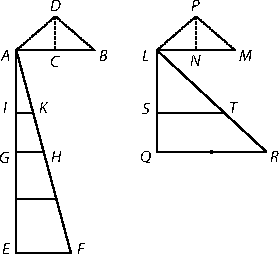
\includegraphics[width=0.47\textwidth]{gesamttex/edit_VIII,3/images/LH_37_05_045-046_d3.pdf}}%
  \vspace{0.5em}
  \centerline{\lbrack\textit{Fig.~3}\rbrack}%
  \label{LH_37_05_046r_Fig.3}%
%  \vspace{1.5em}%
\newpage
\pstart
\noindent sunt in quovis momento temporis \textit{LQ}%
\protect\index{Sachverzeichnis}{momentum temporis}
exprimemus ordinatis \textit{ST}.
Quoniam autem spatium percursum repraesentatur
%
\edtext{area trilinea \textit{AEF}%
\protect\index{Sachverzeichnis}{area trilinea}%
}{%
\lemma{area}\Bfootnote{%
\textit{(1)}~\textit{AEF}
\textit{(2)}~trilinea \textit{AEF}%
~\textit{L}}}
%
vel \textit{LQR},
et spatium%
\protect\index{Sachverzeichnis}{spatium percursum}
utrobique idem est,
erunt aequalia trilinea \textit{AEF} et
%
\edtext{\textit{LQR}.%
\protect\index{Sachverzeichnis}{trilineum}
Quod si fingamus esse triangula,%
\protect\index{Sachverzeichnis}{triangulum}%
}{%
\lemma{\textit{LQR}.}\Bfootnote{%\hspace{-0,5mm}
\textit{(1)}~Sunt enim similia sed nec aliud inter
\textit{(2)}~Quod si fingamus esse triangula,%
~\textit{L}}}
%
quoniam lineae \textit{AHF}, \textit{LTR}
sic satis solent accedere
%
\edtext{rectis,
habetur propositum.%
\protect\index{Sachverzeichnis}{propositum}
Nempe sit \textit{AG}}{%
\lemma{rectis,}\Bfootnote{%
\textit{(1)}~cum potest
\textit{(2)}~habetur propositum.
\textit{(a)}~Nam
\textit{(b)}~Nempe sit \textit{AG}%
~\textit{L}}}
%
(\protect\vphantom)%
dimid. \textit{AE}%
\protect\vphantom()
aeq. \textit{LQ},
et ei respondens ordinata
seu celeritas \textit{GH}.%
\protect\index{Sachverzeichnis}{celeritas restitutionis}
Jam \textit{AEF} aeq.
%
\edtext{\textit{LQR}.
Ergo \textit{LQ} in \textit{QR}}{%
\lemma{\textit{LQR}}\Bfootnote{%\hspace{-0,5mm}
\textit{(1)}~, seu
\textit{(2)}~. Ergo
\textit{(a)}~\textit{LQ} in \textit{QR}
\textit{(b)}~\textit{LQ} in \textit{QR}%
~\textit{L}}}
%
aequ. bis \textit{LQ}
%
\edtext{in \textit{EF}.
Ergo \textit{QR}}{%
\lemma{in}\Bfootnote{%
\hspace{-0,5mm}\textit{EF}.
\textit{(1)}~Ergo \textit{EF}
\textit{(2)}~Ergo \textit{QR}%
~\textit{L}}}
%
aequ. bis \textit{EF}.
Sed \textit{EF} aeq. bis \textit{GH},
ergo \textit{QR} aequ. quater \textit{GH}.
\pend%
   %\newpage%
%%
%%
\pstart%
Sed si
%
\edtext{\textit{AHF} vel \textit{LTR}%
}{%
\lemma{\textit{AHF} vel \textit{LTR}}\Cfootnote{%
Siehe das Diagramm \lbrack\textit{Fig.~4}\rbrack\
auf S.~\pageref{LH_37_05_046r_Fig.4}.}}
%
alia sit a recta%
\lbrack,\rbrack\
non ita accurate res
%
\edtext{procedit.
Nam ponamus
ordinatas \textit{IK}
esse ut quadrata
ipsarum \textit{AI}.
%
%
\edtext{}{%
{\xxref{LH_37_05_046r_Schlussmarg-1}{LH_37_05_046r_Schlussmarg-2}}%
{\lemma{\textit{Am Rand:}}\Afootnote{%
Possumus \textit{a} considerare
ut paulo ante dixi,\textsuperscript{\lbrack a\rbrack}
motum puncti\textsuperscript{\lbrack b\rbrack}%
\protect\index{Sachverzeichnis}{motus puncti repraesentans motum chordae}
\textit{D} ad \textit{C} vel \textit{P} ad \textit{N},
ut repraesentantem motum totius chordae,%
\protect\index{Sachverzeichnis}{motus chordae}
transferendo in ipsum summam motuum reliquorum%
\protect\index{Sachverzeichnis}{summa motuum reliquorum}
ut paulo ante dictum,\textsuperscript{\lbrack c\rbrack}
cum sit centrum grav. reliquorum punctorum%
\protect\index{Sachverzeichnis}{centrum gravitatis chordae}
maneatque in motu.%
\newline\vspace{-0.5em}%
\newline%
{\footnotesize%
\textsuperscript{\lbrack a\rbrack}~dixi:
S.~\refpassage{LH_37_05_046r_antedixi-1}{LH_37_05_046r_antedixi-2}.
%
\quad
\textsuperscript{\lbrack b\rbrack}~puncti
\textit{(1)}~\textit{C} vel \textit{N},
\textit{(2)}~\textit{D} ad \textit{C} vel \textit{P} ad \textit{N},%
~\textit{L}
%
\quad
\textsuperscript{\lbrack c\rbrack}~dictum:
S.~\refpassage{LH_37_05_045r_antedictum-1}{LH_37_05_045r_antedictum-2}.
Vermutlich aber verweist Leibniz vielmehr auf N.~\ref{RK60353}, S.~\refpassage{LH_37_05_180_utpunctumunum-1}{LH_37_05_180_utpunctumunum-2}.%
}}}}%
%
\edlabel{LH_37_05_046r_Schlussmarg-1}%
Sit
\textit{EF} in $a = AE.\text{qu},$
et
\textit{QR} in $b = LQ.\text{quad}.$%
\edlabel{LH_37_05_046r_Schlussmarg-2}
%
$\displaystyle AEFHA = \frac{1}{3}AEF = \frac{1}{3}AE^3\! : a,$
et $\displaystyle LQRTL = \frac{1}{3}LQR = \frac{1}{3}LQ^3\! : b.$%
}{%
\lemma{procedit.}\Bfootnote{%
\textit{(1)}~Sit enim
\textit{(2)}~Nam ponamus ordinatas
\textit{(a)}~\textbar~\textit{ST} \textit{erg.}~%
\textbar\ esse ut quadrat
\textit{(b)}~\textit{IK}, esse % ut quadrata ipsarum 
\lbrack...\rbrack\ \textit{AI}. Sit
\textit{(aa)}~\textit{EF}.qu $\stackrel{(1)}{=}$
\textit{(bb)}~\textit{EF} in $a = AE.\text{qu},$ et
\textit{(aaa)}~$QR = LQ$ in
\textit{(bbb)}~\textit{QR}.qu $\stackrel{(2)}{=} LQ$ in \textit{b}
\textit{(ccc)}~\textit{QR} in $b = LQ$ quad.
\textit{(aaaa)}~$\displaystyle AEP = \frac{1}{3}EF^3\! : a.$ $\displaystyle LQR = \frac{1}{3}$
\textit{(bbbb)}~$\displaystyle AEFHA = \frac{1}{3}AEF$ % $= \displaystyle\frac{1}{3}AE^3 : a,$ et $LQRTL = \displaystyle\frac{1}{3}LQR $
\lbrack...\rbrack\ $= \displaystyle\frac{1}{3}LQ^3\! : b.$%
~\textit{L}}}
%
Jam
$AEFHA
\edtext{= 
LQRTL.$
Ergo
$AE^3\! : a = LQ^3\! : b.$%
}{%
\lemma{$=\, LQRTL$.}\Bfootnote{%\hspace{-0,5mm}
\textit{(1)}~\textbar~Ergo \textit{streicht Hrsg.}~%
\textbar\ \textit{AE}
\textit{(2)}~Ergo $AE^3\! : a = LQ^3\! : b.$%
~\textit{L}}}
%
Sed $AE = \text{bis}\;LQ.$
Ergo $8b \cdot LQ^3\,=$
%
\edtext{\lbrack$a \cdot LQ^3$\rbrack.}{%
\lemma{$a \cdot LQ^3a$}\Bfootnote{%
\textit{L~ändert Hrsg.}}}
%
Ergo
$8 = a : b$
seu
$a = 8b.$
Et
$\displaystyle\frac{1}{3}\, \text{bis}\, LQ$ in \textit{EF}
(\protect\vphantom)%
id est \textit{AEFHA}%
\protect\vphantom()
aequ.
$\displaystyle\frac{1}{3}LQ$ in \textit{QR}.
Ergo
$\text{bis}\,EF = QR.$
Sed
\textit{GH} in \textit{a}
seu \textit{GH} in 8\textit{b}
aeq. \textit{AG}.qu.
aeq. \textit{LQ}.qu.,
et \textit{QR} in $b = LQ.\text{qu.}$
Ergo
8\textit{GH} aequ. \textit{QR}
seu
\textit{QR} foret octupla \textit{GH}.%
\pend%
%
\pstart%
Idem sic ostenditur.
Bis $EF = QR.$
Ergo
bis $AE.\text{qu.} : a = LQ.\text{qu.} : b$
seu $AE = \text{bis}\;LQ.$
Ergo
bis$\cdot$quater $LQ.\text{qu.} : a = LQ.\text{qu.} : b.$
Ergo rursus
%
\edtext{\lbrack$8b = a$\rbrack.}{%
\lemma{$8a = b$}\Bfootnote{%
\textit{L~ändert Hrsg.}}}
%
Hinc si sit verum experimentum%
\protect\index{Sachverzeichnis}{experimentum}
exacte cum recta lineam ut \textit{AHF} valde convenire.%
\pend%
\newpage
 %\vspace{1.5em}%	% Diagramm Fig.~4
  \centerline{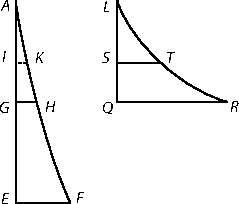
\includegraphics[width=0.44\textwidth]{gesamttex/edit_VIII,3/images/LH_37_05_045-046_d4.pdf}}%
  \vspace{0.5em}
  \centerline{\lbrack\textit{Fig.~4}\rbrack}%
  \label{LH_37_05_046r_Fig.4}%
 \count\Bfootins=1200
\count\Afootins=1200
\count\Cfootins=1200
%
%
%
%%%% Ende des Textes auf Bl. 46r
%
%
%